\documentclass[a4paper, 12pt, finnish]{beamer}
\usepackage{babel}
\usepackage[utf8]{inputenc}
\usepackage[T1]{fontenc}
\usepackage{amsmath}
\usetheme{Copenhagen}

\title{Paikalliset hajautetut verkkoalgoritmit}
\author{Mika Laitinen}
\date{\today}

\begin{document}

\begin{frame}[plain]
    \titlepage
\end{frame}

\begin{frame}{Taustaa}
    \begin{itemize} 
        \item Tyypillisesti tietojenkäsittelytieteessä algoritmit pyritään kehittämään laskennallisesti nopeiksi
        \begin{itemize}
            \item Yksi kokonaisuus ratkaisee ongelmaa, ja kommunikaatiokustannukset ovat pieniä
        \end{itemize} 
        \pause
        \item Suuria verkkoja, kuten Internetiä, ihmisaivoja tai sensoriverkkoja on vaikeaa tai mahdotonta hallita keskitetysti
        \begin{itemize}
            \item Perinteisiin ongelmiin verrattuna kommunikaatiokustannukset ovat merkittävät
            \item Laskenta halpaa verrattuna kommunikaatioon
        \end{itemize}
        \pause
        \item Voidaanko tällaisia ongelmia lähestyä erilaisella mallilla?
    \end{itemize} 
\end{frame}

\begin{frame}{Mallit}
    \begin{itemize}
        \item Idea: laitetaan jokaiseen verkon solmuun prosessori, jotka voivat kommunikoida vain naapuriprosessoreidensa kanssa
        \begin{itemize}
            \item Suuntaamaton verkko, jossa prosessorit ovat naapureita keskenään, jos niiden välillä on kaari
        \end{itemize}
        \pause
        \item Jokainen prosessori pyrkii ratkaisemaan paikallisesti oman osansa koko verkkoa koskevasta ongelmasta
        \pause
        \item Algoritmin suorituksen alussa jokaiselle prosessorille annetaan rajattu määrä informaatiota
        \begin{itemize}
            \item Prosessori tietää verkon koostumuksen vain paikallisesti
        \end{itemize}
        \pause
        \item Kaikki prosessorit ajavat samaa algoritmia
    \end{itemize}
\end{frame}

\begin{frame}{Mallit}
    \begin{center} 
        \includegraphics[width=0.8\textwidth]{Diagram2n.jpeg} 
    \end{center} 
\end{frame}

\begin{frame}{Mallit}
    \begin{itemize}
        \item Mitä informaatiota prosessoreille täytyy antaa?
        \pause
        \item Vähimmäisvaatimus: naapureiden kanssa on voitava kommunikoida
        \item Ensimmäinen ajatus: määritellään, että prosessoreille annetaan naapuriprosessorit järjestettynä listana
        \pause
        \item Ongelma: prosessorit ajavat samaa algoritmia, ja jos ne ovat symmetrisessä tilanteessa keskenään, niiden täytyy tuottaa sama tulos!
    \end{itemize}
\end{frame}

\begin{frame}{Mallit}
    \begin{itemize}
        \item Symmetrisessa tilanteessa algoritmit saavat saman informaation
        \begin{itemize}
            \item Deterministinen algoritmi tuottaa tällöin saman vastauksen
            \item Symmetria on pakko rikkoa, tai joitain ongelmia ei voida ratkaista
        \end{itemize}
    \end{itemize}
    \begin{center}
        \includegraphics[width=0.4\textwidth]{symmetria.jpeg} 
    \end{center}
\end{frame}

\begin{frame}{Mallit}
    \begin{itemize}
        \item Symmetrian voi rikkoa satunnaisuuden avulla, mutta determinismistä ei ole pakko luopua
        \item Yksinkertainen muutos malliin: annetaan jokaiselle prosessorille uniikki tunnistenumero
        \item $\Rightarrow$ Kaikki ratkeavat ongelmat voidaan ratkaista uudella mallilla $O(diam(G))$ kommunikaatiokierroksessa
    \end{itemize}
\end{frame}

\begin{frame}{Mallit}
    \begin{center} 
        \includegraphics[width=0.5\textwidth]{Diagram1.jpeg} 
    \end{center} 
\end{frame}

\begin{frame}{Cole-Vishkin: verkon 6-väritys}
    \begin{itemize}
        \item Verkon väritys: löydettävä jokaiselle solmulle väri (kokonaisluku) siten, että millään solmun naapurilla ei ole samaa väriä
        \item Mitä vähemmän värejä, sen parempi
        \item Colen-Vishkinin algoritmilla voidaan 6-värittää suunnattu verkko, jossa jokaisella solmulla on maksimissaan yksi jälkeläinen
    \end{itemize}
\end{frame}

\begin{frame}{Cole-Vishkin: verkon 6-väritys}
    \begin{center} 
        \includegraphics[width=0.5\textwidth]{Diagram3.jpeg} 
    \end{center} 
\end{frame}

\begin{frame}{Cole-Vishkin: verkon 6-väritys}
    \begin{itemize}
        \item Verkon väritys: löydettävä jokaiselle solmulle väri (kokonaisluku) siten, että millään solmun naapurilla ei ole samaa väriä
        \item Mitä vähemmän värejä, sen parempi
        \item Colen-Vishkinin algoritmilla voidaan 6-värittää suunnattu verkko, jossa jokaisella solmulla on maksimissaan yksi jälkeläinen
        \begin{itemize}
            \item Jokaisella solmulla on myös oltava alussa väri
            \item Prosessoreille annetut tunnistenumerot käyvät alkuväreinä
        \end{itemize}
        \item Lopullisessa verkossa solmuilla voi olla vain kuusi erillistä väriä
    \end{itemize}
\end{frame}

\begin{frame}{Cole-Vishkin: verkon 6-väritys}
    \begin{center} 
        \includegraphics[width=0.5\textwidth]{Diagram4.jpeg} 
    \end{center} 
\end{frame}

\begin{frame}{Cole-Vishkin: verkon 6-väritys}
    \begin{center} 
        \includegraphics[width=0.5\textwidth]{Diagram5.jpeg} 
    \end{center} 
\end{frame}

\begin{frame}{Cole-Vishkin: verkon 6-väritys}
    \begin{center} 
        \includegraphics[width=0.7\textwidth]{Diagram6.jpeg} 
    \end{center} 
\end{frame}

\begin{frame}{Cole-Vishkin: verkon 6-väritys}
    \begin{center} 
        \includegraphics[width=0.8\textwidth]{Diagram7.jpeg} 
    \end{center} 
\end{frame}

\begin{frame}{Cole-Vishkin: verkon 6-väritys}
    \begin{center} 
        \includegraphics[width=0.5\textwidth]{Diagram8.jpeg} 
    \end{center} 
\end{frame}

\begin{frame}{Cole-Vishkin: verkon 6-väritys}
    \begin{center} 
        \includegraphics[width=0.75\textwidth]{Diagram9.jpeg} 
    \end{center} 
\end{frame}

\begin{frame}{Cole-Vishkin: verkon 6-väritys}
    \begin{center} 
        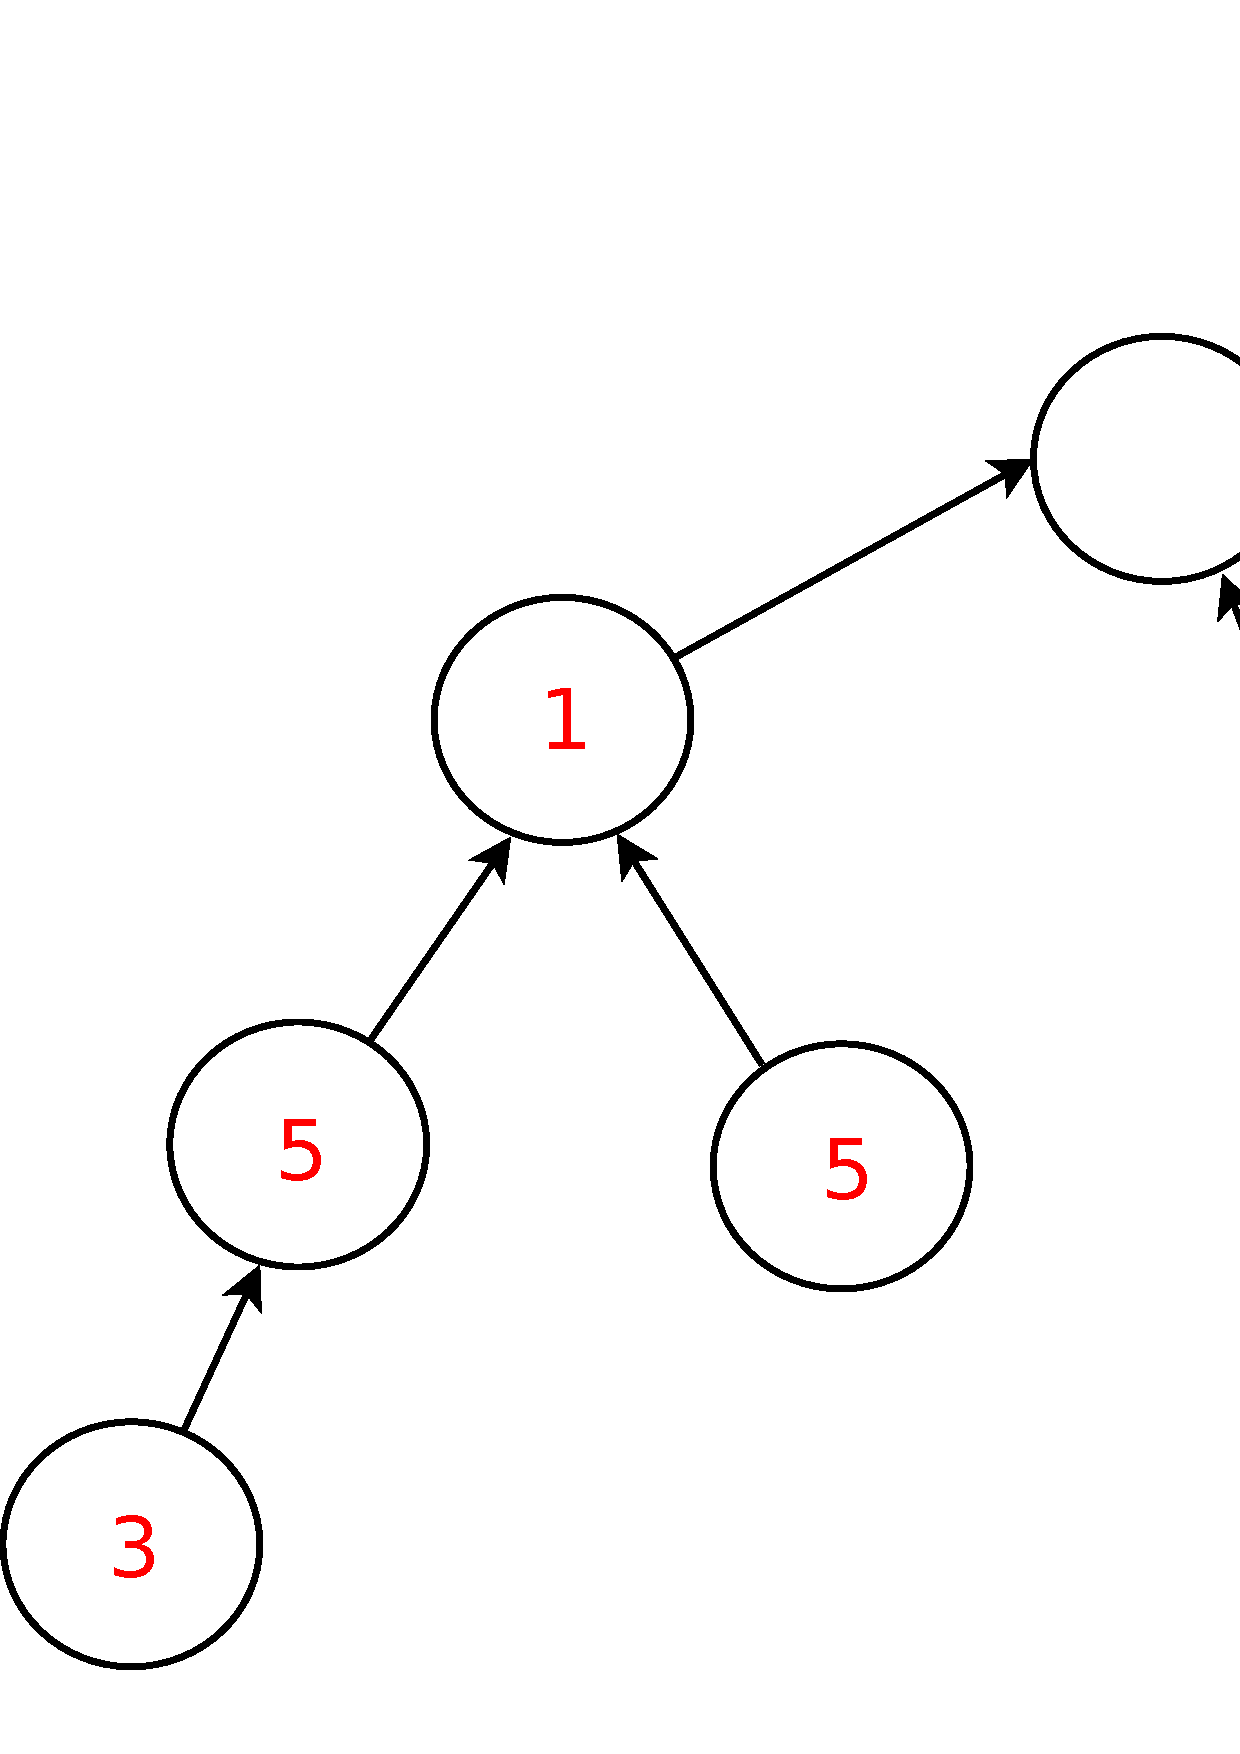
\includegraphics[width=0.5\textwidth]{Diagram10.jpeg} 
    \end{center} 
\end{frame}

\begin{frame}{Cole-Vishkin: verkon 6-väritys}
    \begin{center} 
        \includegraphics[width=0.5\textwidth]{Diagram11.jpeg} 
    \end{center} 
\end{frame}

\begin{frame}{Cole-Vishkin: verkon 6-väritys}
    \begin{center} 
        \includegraphics[width=0.75\textwidth]{Diagram12.jpeg} 
    \end{center} 
\end{frame}

\begin{frame}{Cole-Vishkin: verkon 6-väritys}
    \begin{itemize} 
        \item Jokaisella kierroksella värien määrä vähenee ainakin logaritmisesti
        \item Kommunikaatiokierroksia tarvitaan siis $O(\log^* N)$ kappaletta, jossa $N$ on prosessorien määrä
        \item Algoritmi toimii, sillä yksikään naapuri ei voi valita kommunikaatiokierroksen jälkeen samaa väriä kuin prosessori itse valitsee, joten algoritmin jokaisessa vaiheessa väritys on käypä
    \end{itemize} 
\end{frame}

\begin{frame}{Käytäntö}
    \begin{itemize}
        \item Käsiteltävän tiedon määrä kasvaa jatkuvasti
        \begin{itemize}
            \item Paikalliset algoritmit pystyvät ratkaisemaan ainakin joitain ongelmia hyvin nopeasti 
            \item Prosessoriverkko konstruoitava ennen laskentaa
        \end{itemize}
        \item Joitain rohkaisevia tutkimustuloksia, sekä biologisia esimerkkejä, kuten aivotoiminta
        \item Sensoriverkot, mobiiliverkot
    \end{itemize}
\end{frame}

\begin{frame}{Kiitos huomiostanne}
    \begin{itemize}
        \item Kysymyksiä?
    \end{itemize}
\end{frame}
\end{document}
